\documentclass[12pt]{article}
\usepackage{paper,math}
\usepackage{natbib}
\usepackage{float}
\usepackage{multibib}
\usepackage{threeparttable}
\newcites{W}{Planned Further Reading}
% titlepage.tex - Simple thesis-style title page

% Use basic LaTeX variable storage
\def\thesistitletext{}
\def\thesisauthortext{}
\def\advisortext{}
\def\depttext{Economics}
\def\deptprefixtext{Department of}
\def\thesisdatetext{\today}
\def\acknowledgementstext{}

% Simple commands to set variables
\newcommand{\thesistitle}[1]{\def\thesistitletext{#1}}
\newcommand{\thesisauthor}[1]{\def\thesisauthortext{#1}}
\newcommand{\advisor}[1]{\def\advisortext{#1}}
\newcommand{\department}[1]{\def\depttext{#1}}
\newcommand{\departmentprefix}[1]{\def\deptprefixtext{#1}}
\newcommand{\thesisdate}[1]{\def\thesisdatetext{#1}}
\newcommand{\thesisacknowledgements}[1]{\def\acknowledgementstext{#1}}

% Thesis title page (page 1) - no abstract
\newcommand{\makethesistitle}{%
  \thispagestyle{empty}
  
  % Temporarily adjust margins
  \newgeometry{margin=1in, top=0.75in, bottom=1in}
  
  % Single spacing
  \begin{spacing}{1.0}
  
  \begin{center}
    \vspace*{0.5in}
    
    % Title
    {\huge\bfseries \thesistitletext}
    
    \vspace{0.8in}
    
    % Author
    {\Large \thesisauthortext}
    
    \vspace{0.3in}
    
    % Advisor
    {\large Advisor: \advisortext}
    
    \vspace{0.8in}
    
    % Institution
    {\large
      Submitted to the \\[0.2in]
      Distinguished Majors Program \\[0.1in]
      \deptprefixtext{} \depttext \\[0.1in]
      University of Virginia
    }
    
    \vspace{1.0in}
    
    % Date
    {\large \thesisdatetext}
    
  \end{center}
  
  \end{spacing}
  
  % Restore geometry
  \restoregeometry
  
  \clearpage
}

% Academic paper format page (page 2) - with abstract
\newcommand{\makeacademicpage}{%
  \newpage
  \thispagestyle{empty}
  
  % Use paper.sty's built-in title formatting but with footnote without marker
  \begin{center}
    {\huge\bfseries \thesistitletext%
    \renewcommand{\thefootnote}{}%  % This removes the footnote marker
    \footnote{\acknowledgementstext}%
    \renewcommand{\thefootnote}{\arabic{footnote}}%
    \setcounter{footnote}{0}}
    \par\vspace{2em}
    {\Large \thesisauthortext}
    \par\vspace{1em}
    {\large\scshape\color{zinc700} \thesisdatetext}
  \end{center}
  
  \vspace{2em}
  
  % Add Abstract heading
  \begin{center}
  \end{center}
  \vspace{2em}
  
  % This is where the abstract content will be added
 
    % Reset page counter so next page starts at 1
  \setcounter{page}{1}
}

% Statement/declaration page
\newcommand{\makestatements}{%
  \newpage
  \thispagestyle{empty}
  \begin{spacing}{1.0}
  
  \vspace*{0.5in}
  
  \noindent I hereby declare that I am the sole author of this thesis.
  
  \vspace{0.4in}
  
  \noindent I authorize University of Virginia to lend this thesis to other 
  institutions or individuals for the purpose of scholarly research.
  
  \vspace{0.8in}
  
  \hfill
  \begin{minipage}{3in}
    \hrulefill \\
    \thesisauthortext
  \end{minipage}
   
  \vspace{1.0in}
  
  \noindent I further authorize University of Virginia to reproduce this thesis by photocopying or by
  other means, in total or in part, at the request of other institutions or individuals for the
  purpose of scholarly research.
  
  \vspace{0.8in}
  
  \hfill
  \begin{minipage}{3in}
    \hrulefill \\
    \thesisauthortext
  \end{minipage}
  
  \end{spacing}
  \clearpage
} 

% Set thesis information
\thesistitle{Eviction Moratoria and the Flow of Rehousing: Evidence from the COVID-19 Era}
\thesisauthor{Mary Edith Plunkett}
\advisor{Dr. Lee Lockwood}
\department{Economics}
\departmentprefix{Department of}
\thesisdate{\today}
\thesisacknowledgements{\noindent Email: \href{mailto:zjh6sn@virginia.edu}{zjh6sn@virginia.edu}. I would like to thank my advisor and family...
}

\hypersetup{
  pdftitle = {Eviction Moratoria and the Flow of Rehousing: Evidence from the COVID-19 Era},
  pdfauthor = {Mary Edith Plunkett},
}

% Conditionally display thoughts
\booltrue{INCLUDECOMMENTS}

%%%%%%%%%%%%%%%%%%%%%%%%%%%%%%%%%%
\begin{document}
%%%%%%%%%%%%%%%%%%%%%%%%%%%%%%%%%%

% Page 1: Thesis title page (no abstract)
 % \makethesistitle

%%%%%%%%%%%%%%%%%%%%%%%%%%%%%%%%%%
% Page 2: Academic format with title, author, and abstract  
\makeacademicpage
\noindent This paper examines whether COVID-19 eviction moratoria unintentionally reduced the capacity of homelessness systems to rehouse people. When moratoria sharply suppressed eviction filings, they also reduced turnover in the lowest-cost rentals—the very units rapid-rehousing programs rely on. The project assembles a 2016–2023 panel of HUD Continuums of Care (CoC), merged with the Princeton Eviction Lab's Eviction Tracker data and COVID-19 Housing Policy Scorecards and uses a dose–response difference-in-differences model to exploit variation in moratorium timing and stringency across localities. I expect stronger or longer moratoria to reduce inflow and outflow rates and increase average time homeless—evidence of a turnover-induced bottleneck. If confirmed, the results would show that eviction prevention and homelessness rehousing draw on the same scarce stock of low-cost units. The findings underscore that effective prevention must be paired with expanded affordable supply, reframing homelessness as a dynamic flow equilibrium shaped by housing availability.

\par\vspace{4em}\noindent
{\color{zinc700}Keywords: Housing and Urban Development, Rapid Re-Housing, Welfare Policy} 
\par\noindent
{\color{zinc700}JEL-Classification: I80} 
%%%%%%%%%%%%%%%%%%%%%%%%%%%%%%%%%%

\newpage

% Paper ------------------------------------------------------------------------
% ------------------------------------------------------------------------------
\section{Introduction}
% ------------------------------------------------------------------------------
Evictions and homelessness are often treated as distinct social problems, governed by separate policy regimes and studied in largely separate literatures. Evictions are typically analyzed as shocks to individual households—events that increase housing instability, disrupt employment, and raise the risk of subsequent hardship. Homelessness, by contrast, is commonly framed as a problem of insufficient services or inadequate funding within shelter and rehousing systems. Yet in practice, both phenomena are embedded in the same low-income housing ecosystem, and policy interventions aimed at one may have unintended consequences for the other.

This paper studies the relationship between eviction prevention and the flow of rehousing from homelessness. In particular, it asks whether policies that suppress evictions—while protecting tenants from displacement—also alter the availability of low-cost rental units used to rehouse people experiencing homelessness. If homelessness systems rely on a steady stream of housing turnover at the bottom of the rental market, then disruptions to that turnover may create downstream congestion, lengthening homelessness spells even when program effectiveness remains unchanged. Understanding this mechanism is central to evaluating housing policy: it speaks not only to how many people become homeless, but to how quickly systems are able to help people exit homelessness once they enter.

 Answering this question is challenging for several reasons. First, homelessness is a dynamic phenomenon governed by flows, not just stocks. Standard point-in-time counts obscure the distinction between changes in inflows into homelessness and changes in the duration of homelessness, even though these margins have very different policy implications. A decline in homelessness may reflect fewer people entering shelters, faster rehousing, or both; similarly, congestion may manifest as longer stays even if entry rates fall. Disentangling these mechanisms requires data that track system throughput over time rather than static snapshots.

Second, eviction prevention policies are difficult to evaluate causally. Evictions respond endogenously to local economic conditions, housing market tightness, and policy environments, all of which also directly affect homelessness. Moreover, large-scale eviction interventions—such as the COVID-19 eviction moratoria—coincided with other unprecedented shocks, including public health restrictions, emergency fiscal transfers, and changes in shelter operations. Isolating the effects of suppressed eviction activity on rehousing outcomes therefore requires a research design that can separate policy-induced variation in eviction exposure from broader pandemic-related trends.

This paper addresses these challenges by studying eviction moratoria during the COVID-19 pandemic as a natural experiment in housing-market disruption. It examines whether areas that experienced more intense or longer-lasting eviction suppression also experienced slower rehousing from homelessness, consistent with a congestion mechanism operating through reduced vacancy turnover. Using administrative data from HUD’s System Performance Measures combined with variation in moratorium timing and scope across states, the paper estimates how eviction prevention policies affected homelessness inflows, exits, and duration.

The analysis is guided by a simple dynamic framework that conceptualizes homelessness systems as queues. Individuals enter homelessness at a rate determined by economic shocks and housing instability, and they exit at a rate determined by the availability of housing placements and service capacity. In this framework, the key parameters of interest are the inflow rate into homelessness and the outflow rate from homelessness into permanent housing. Policies that reduce evictions may lower inflows, but they may also affect outflows by altering the supply of low-cost vacant units. When housing turnover slows, exits may fall even if programs remain equally effective conditional on available placements.

To study these dynamics, the paper assembles a panel of Continuums of Care (CoCs)—HUD-defined regional homelessness systems—from 2016 to 2023. Homelessness outcomes are drawn from HUD’s System Performance Measures, which report annual data on total exits, exits to permanent housing, average days homeless, and successful exit rates. Eviction activity is measured using data from the Princeton Eviction Lab, aggregated to align with CoC geographies. Policy exposure is captured using state-level eviction moratorium timing and scope, converted into a continuous measure of annual moratorium intensity.

The key empirical challenge is to isolate the effect of eviction suppression on homelessness outcomes amid overlapping shocks. The paper employs a dose–response difference-in-differences design that exploits variation across states in both the duration and stringency of eviction moratoria. CoC fixed effects control for time-invariant differences in shelter capacity and baseline housing conditions, while year fixed effects absorb national shocks such as stimulus payments and pandemic trends. An event-study specification provides a diagnostic check for pre-trends and illustrates how homelessness outcomes evolve around the introduction and expiration of moratoria.




% ------------------------------------------------------------------------------
\section{Literature Review}
% ------------------------------------------------------------------------------
This project sits at the intersection of three literatures: (i) the determinants and dynamics of homelessness, (ii) eviction and housing instability as drivers of homelessness risk, and (iii) policy interventions that alter housing market frictions and the flow of households into and out of homelessness.

\subsection{Homelessness Dynamics and Measurement}

A central insight in the economics literature is that homelessness is best understood as a dynamic process governed by both entry into homelessness and exit through rehousing. \citet{oflaherty2019} provides a comprehensive overview of homelessness research, emphasizing the importance of distinguishing between inflows, exits, and durations when analyzing homelessness trends and policy impacts. This perspective motivates the use of administrative data systems, such as HUD’s System Performance Measures (SPM), which allow researchers to observe homelessness as a flow process rather than a static stock.

Early empirical work documented substantial geographic variation in homelessness rates and linked these differences to local economic and housing market conditions. For example, \citet{honigfiler1993} study intercity variation in homelessness and highlight the role of labor market conditions and housing costs. Subsequent research has focused more explicitly on the duration of homelessness spells. \citet{cobbclark2014} show that both individual characteristics and local institutional environments shape how long individuals remain homeless, underscoring the importance of system capacity and rehousing processes.

\subsection{Eviction, Housing Instability, and Homelessness}

Empirically identifying the causal effect of eviction on homelessness is challenging because eviction risk is correlated with unobserved vulnerability and because many households exit housing before formal eviction occurs. Recent work has addressed data limitations through large-scale administrative datasets such as the Eviction Lab, which has enabled systematic measurement of eviction filings across jurisdictions \citep{desmond2018}. This literature motivates the use of policy-induced variation in eviction exposure—rather than individual eviction events—to study downstream homelessness outcomes.

\subsection{Policy Interventions and Homelessness}

A third literature evaluates policy interventions designed to reduce homelessness or mitigate its severity by increasing housing stability and rehousing capacity. A prominent strand of this work studies Housing First and Rapid Re-Housing (RRH) programs, which provide housing assistance with minimal preconditions. Evaluations of Housing First programs consistently find large reductions in chronic homelessness and significant increases in housing stability, primarily through faster exits from homelessness and longer housing retention \citep{tsai2010, tsemberis2004}. Similarly, evidence on Rapid Re-Housing suggests that short-term rental assistance and supportive services can substantially accelerate exits from homelessness, though effects on long-run housing outcomes are more mixed \citep{gubits2016}.

This literature emphasizes that homelessness outcomes are highly responsive to policies that alter exit rates and the duration of homelessness spells, even when inflows remain unchanged. As a result, system-level congestion and average time homeless may shift significantly in response to rehousing policies without large changes in the number of people entering homelessness.


\subsection{Contribution of This Paper}

This paper asks whether eviction suppression during the COVID-19 pandemic altered homelessness system dynamics, with a particular focus on exits from homelessness. Specifically, I ask: did areas experiencing larger declines in eviction activity during 2020–2021 also experience larger declines in total exits from homelessness? And to what extent were changes in exits driven by reduced housing turnover—such as a shortage of available low-rent units for rehousing—rather than by changes in client characteristics, funding levels, or program effectiveness?

To address these questions, the paper contributes to the literature in two primary ways. First, it applies a flow-based perspective to the study of eviction moratoria and homelessness, separately examining inflows into homelessness, exits from homelessness, and the duration of homelessness spells. Second, it exploits variation in the intensity of eviction moratoria within a difference-in-differences framework, using Continuum of Care fixed effects to absorb time-invariant local differences and year fixed effects to net out common shocks. 

% ------------------------------------------------------------------------------
\section{Theoretical Framework}
% ------------------------------------------------------------------------------

I model homelessness as a dynamic system governed by flows into and out of homelessness. Let $\lambda_{st}$ denote the rate at which individuals enter homelessness in state $s$ at time $t$, and let $\mu_{st}$ denote the rate at which individuals exit homelessness through rehousing or other permanent destinations. The stock of individuals experiencing homelessness and the average duration of homelessness depend on the balance between these entry and exit rates. Figure~\ref{fig:queue} illustrates the queuing framework introduced above.

This flow-based perspective clarifies how different policies affect homelessness outcomes. Policies that prevent housing loss, such as eviction moratoria, primarily operate by reducing $\lambda_{st}$, the rate of entry into homelessness. In contrast, policies that expand rehousing capacity or reduce barriers to housing placement—such as Housing First or Rapid Re-Housing programs—operate by increasing $\mu_{st}$, accelerating exits and shortening homelessness spells. Changes in either margin can alter observed homelessness outcomes even if the other margin remains unchanged.

Eviction moratoria therefore have theoretically ambiguous effects on homelessness dynamics. While suppressing formal evictions may reduce immediate entry into homelessness, moratoria may also delay housing transitions, alter landlord behavior, or interact with limited rehousing capacity in ways that affect exits and system congestion. This ambiguity motivates an empirical approach that separately examines inflows, exits, and duration.

This framework guides the empirical analysis by motivating outcome selection and informing the dose–response specification used below. Variation in the intensity of eviction suppression across states and over time may generate proportional or nonlinear changes in entry and exit rates, producing heterogeneous effects across homelessness outcomes.

% ------------------------------------------------------------------------------
\section{Data}
% ------------------------------------------------------------------------------

This paper assembles a panel dataset of U.S. states spanning 2016–2023, combining administrative homelessness data with state-level eviction policy information. The primary unit of observation is the state–year.

\subsection{Homelessness Outcomes}

Data on homelessness dynamics come from the U.S. Department of Housing and Urban Development’s (HUD) System Performance Measures (SPM). These data provide annual measures of homelessness system performance for each Continuum of Care (CoC), including the number of individuals experiencing homelessness for the first time, total exits from homelessness, and the average length of time individuals remain homeless.

Because eviction policy varies at the state level, I aggregate the CoC-level SPM data to the state level. For each state–year observation, I construct the following outcomes:

\begin{itemize}
\item \textbf{First-time homelessness inflows:} total number of individuals entering homelessness for the first time, summed across CoCs within each state.
\item \textbf{Total exits from homelessness:} total number of exits from homelessness programs, summed across CoCs within each state.
\item \textbf{Permanent housing exits:} total number of exits to permanent housing destinations, summed across CoCs.
\item \textbf{Average days homeless:} mean duration of homelessness across CoCs within a state.
\end{itemize}

To account for differences in population across states, inflows and exits are converted to rates per 1,000 residents using annual state population estimates.

\subsection{Eviction Moratoria}

Information on eviction moratoria is drawn from the Princeton Eviction Lab’s COVID-19 Housing Policy Scorecard, which documents the timing, scope, and legal strength of eviction restrictions enacted by U.S. states during the COVID-19 pandemic. The dataset records when state actors—typically governors, courts, or legislatures—restricted specific stages of the eviction process and when those restrictions expired. Because eviction law is procedurally complex, moratoria did not operate as a single uniform policy. Instead, states intervened at different points in the eviction process and with varying degrees of legal strength.

The Eviction Lab dataset distinguishes five primary stages of the eviction process. The first stage is the \textit{initiation of eviction}, which includes the service of notice to quit and the filing of eviction claims in court. The second stage is the \textit{court process}, which includes eviction hearings, court judgments of possession, and procedural deadlines governing eviction cases. The third stage is \textit{enforcement}, in which law enforcement officers execute writs of possession and physically remove tenants from properties. The fourth and fifth stages consist of broader policy supports designed to stabilize housing during the pandemic, including short-term tenant supports and longer-term tenancy preservation measures such as rental assistance programs or restrictions on rent increases.

Importantly, moratoria differed substantially in which of these stages they targeted. Some states prohibited landlords from initiating eviction proceedings by banning notices to quit or the filing of eviction claims. Others allowed cases to be filed but suspended court hearings or delayed judgments. Still others permitted cases to proceed through the court system but prohibited law enforcement from executing eviction orders. Because each stage represents a different point in the eviction pipeline, policies operating at earlier stages tend to provide broader protection for tenants than those operating later in the process. For example, prohibiting eviction filings prevents cases from entering the court system entirely, while suspending enforcement delays removal but may still allow eviction judgments to accumulate.

In addition to these stage-based distinctions, many policies included limitations that affected their effective strength. Some restrictions applied only to tenants who could demonstrate financial hardship related to COVID-19. Others applied only to evictions filed for nonpayment of rent rather than to all causes of eviction. In contrast, the strongest protections prohibited eviction filings or enforcement actions except in narrowly defined emergency cases. These design differences imply that two states with moratoria in place at the same time could nevertheless provide substantially different levels of protection to tenants.

To capture this variation, the Eviction Lab constructs a composite policy index—the Housing Policy Scorecard—that summarizes eviction protections using a weighted scoring system. The scorecard groups policies into five categories corresponding to stages of the eviction process and broader housing stability measures: initiation of eviction, court process, enforcement of eviction orders, short-term tenant supports, and tenancy preservation measures. Each category contributes a different share to the overall score based on the expected importance of that stage for preventing housing loss. Initiation of eviction receives the largest weight, accounting for 40 percent of the total score, because preventing eviction filings directly blocks cases from entering the legal system. Court process and enforcement measures each account for 15 percent of the score, while short-term supports and longer-term tenancy preservation policies account for 10 percent and 20 percent, respectively.

Within each category, the scorecard assigns points based on the presence of specific policies and their comprehensiveness. For example, within the initiation category, prohibiting eviction filings for nonpayment of rent carries greater weight than restricting filings only for tenants experiencing COVID-19 hardship, while the most comprehensive protection—prohibiting all non-emergency eviction filings—receives the highest weight. Similar hierarchies apply in other categories: for instance, prohibiting all eviction enforcement actions is treated as stronger than prohibiting enforcement only in nonpayment cases. The final score ranges from zero to five, where higher values indicate stronger and more comprehensive eviction protections.

Rather than classifying states using a simple binary indicator for whether a moratorium was in place, I construct continuous measures that capture both the \textit{duration} and \textit{strength} of eviction restrictions. The first measure counts the number of days in each year during which any eviction prohibition was active. The second measure uses the Eviction Lab scorecard to capture the legal strength of eviction protections. I then construct a composite \textit{moratorium intensity} measure that multiplies the duration of active protections by the policy scorecard. This measure captures the effective ``dose’’ of eviction suppression experienced by a state in a given year, allowing states with longer or stronger moratoria to receive larger policy values. Finally, I construct measures capturing the number of days in which eviction protections were active at each of the five stages. These variables allow heterogeneity analysis to explore whether moratoria operating earlier or later in the eviction pipeline have different effects on homelessness outcomes.

\subsection{Descriptive Statistics}

\begin{table}
\centering
\begin{threeparttable}
\caption{Pre-COVID Summary Statistics}
\label{tab:summary_stats}
\begin{tabular}{lllllll}
\toprule
 & \multicolumn{2}{c}{Full Sample (N = 208)} & \multicolumn{2}{c}{Control (N = 32)} & \multicolumn{2}{c}{Treatment (N = 176)} \\
 & Mean & SD & Mean & SD & Mean & SD \\
\midrule
Inflow & 264.153 & 163.107 & 199.340 & 99.692 & 275.937 & 169.707 \\
Average Days Homeless & 121 & 98 & 120 & 59 & 121 & 103 \\
Exits & 289.944 & 159.898 & 217.808 & 123.295 & 303.059 & 162.559 \\
Population & 6361550 & 7214528 & 5011173 & 3955948 & 6607073 & 7642039 \\
Renting Population & 2092885 & 2849373 & 1495083 & 1330231 & 2201577 & 3035267 \\
Unemployment Rate & 4.155 & 1.294 & 4.692 & 2.223 & 4.058 & 1.022 \\
\bottomrule
\end{tabular}

\begin{tablenotes}[flushleft]
\footnotesize
\item \textit{Notes:} Inflow refers to the number of individuals entering homelessness per thousand in the population for the first time in a given year, while exits refer to the number of individuals per thousand in the population exiting the homelessness system in that year. Population measures refer to total state population and estimated renting population, respectively.
\end{tablenotes}
\end{threeparttable}
\end{table}

Table~\ref{tab:summary_stats} reports summary statistics for the primary outcomes and control variables used in the analysis using the pre-COVID sample (2016–2019). The table presents statistics for the full sample as well as separately for states that eventually implemented eviction moratoria (“treatment’’) and those that did not (“control’’). Restricting the sample to the pre-policy period allows comparison of baseline characteristics prior to the onset of COVID-19 eviction protections.

Several patterns emerge from the table. States that later implemented eviction moratoria tend to have substantially larger housing markets. The average renting population in treated states is roughly 2.2 million compared to approximately 1.5 million in control states, and treated states also have somewhat larger total populations. These differences suggest that states adopting eviction moratoria were generally larger and more urbanized housing markets, where eviction pressures and housing instability may have been more salient policy concerns.

Homelessness system flows are also larger in treated states. Average inflows and exits from homelessness are higher in the treatment group than in the control group. Because these measures are reported in levels rather than population-adjusted rates, these differences likely reflect the larger populations of treated states rather than systematically higher homelessness risk.

In contrast, the average duration of homelessness appears similar across groups. The mean number of days individuals experience homelessness is nearly identical between treated and untreated states in the pre-policy period, suggesting that baseline system throughput was broadly comparable across the two groups.

Taken together, these descriptive statistics highlight meaningful structural differences between states that adopted eviction moratoria and those that did not, particularly in the size of their housing markets and homelessness systems. These differences motivate the empirical strategy adopted in the paper. Rather than relying on a simple treated-versus-untreated comparison, the analysis exploits variation in the intensity and duration of eviction protections across states and over time while controlling for state fixed effects.

Figure~\ref{fig:national_trends} plots national totals of homelessness system inflows and exits from 2016 through 2023, along with measures of homelessness duration. Several clear patterns emerge. Prior to the COVID-19 pandemic, exits from the homelessness system consistently exceeded inflows. Between 2016 and 2019, annual exits were roughly 50,000 to 100,000 higher than the number of individuals entering homelessness for the first time. This pattern suggests that, at the national level, homelessness systems were operating in a regime where rehousing flows were sufficient to offset new entries into homelessness.

\begin{figure}
\centering
    \centering
    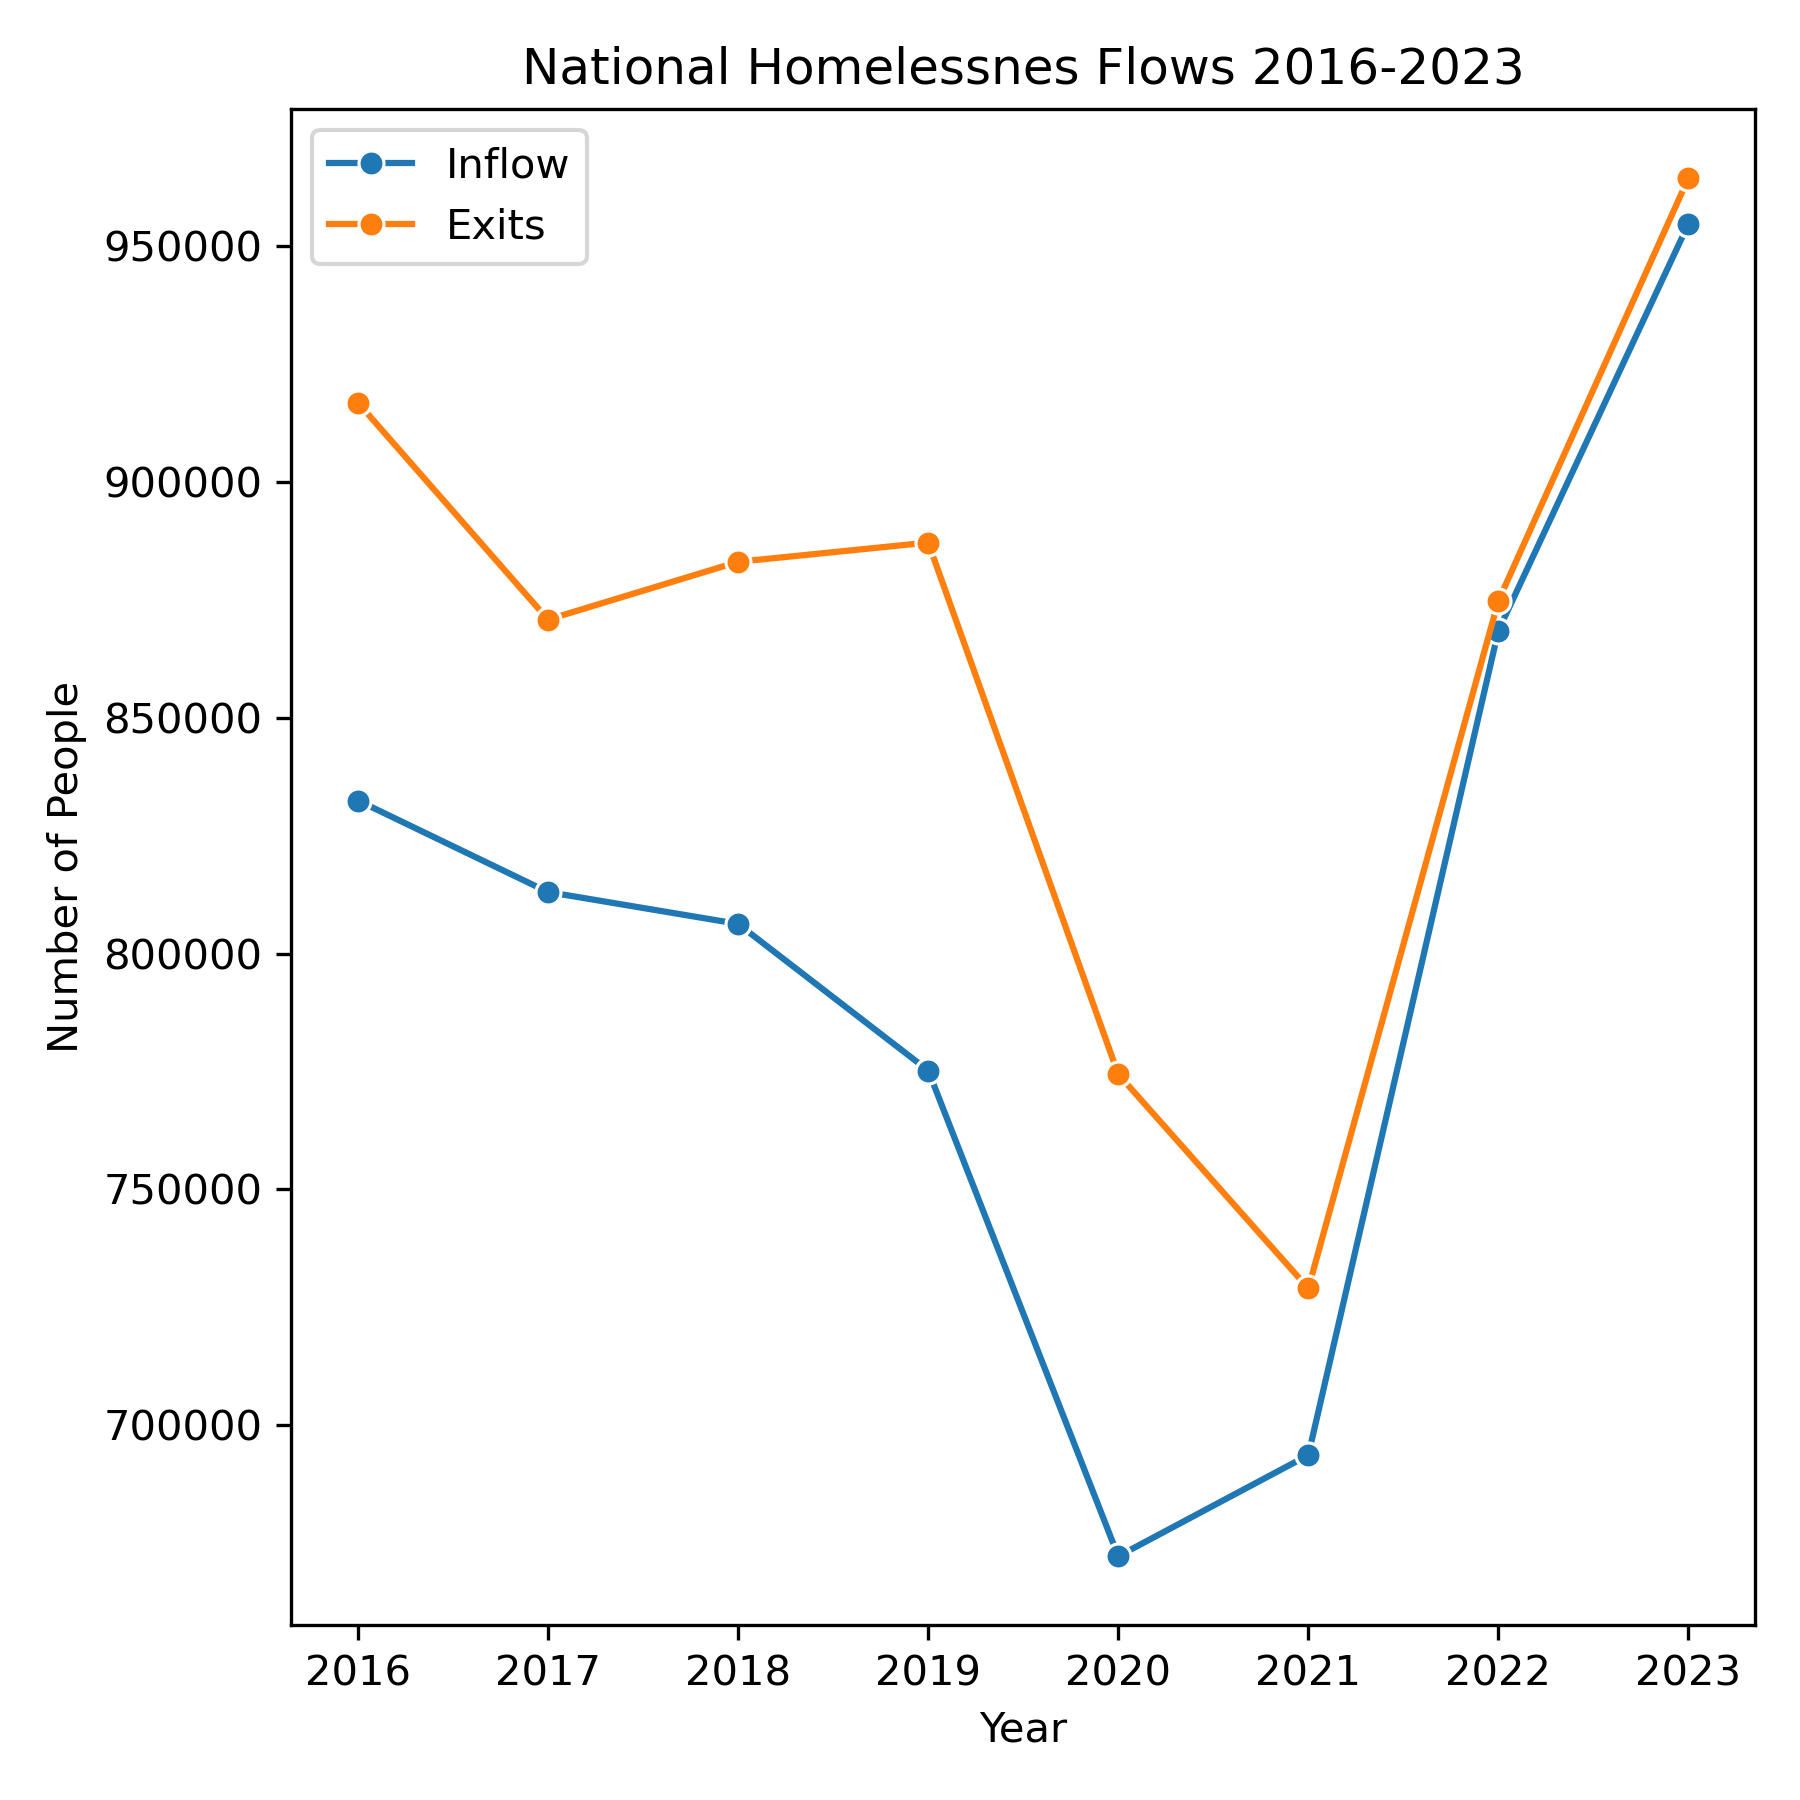
\includegraphics[width=0.48\linewidth]{graphs/homelessness_flows.png}
    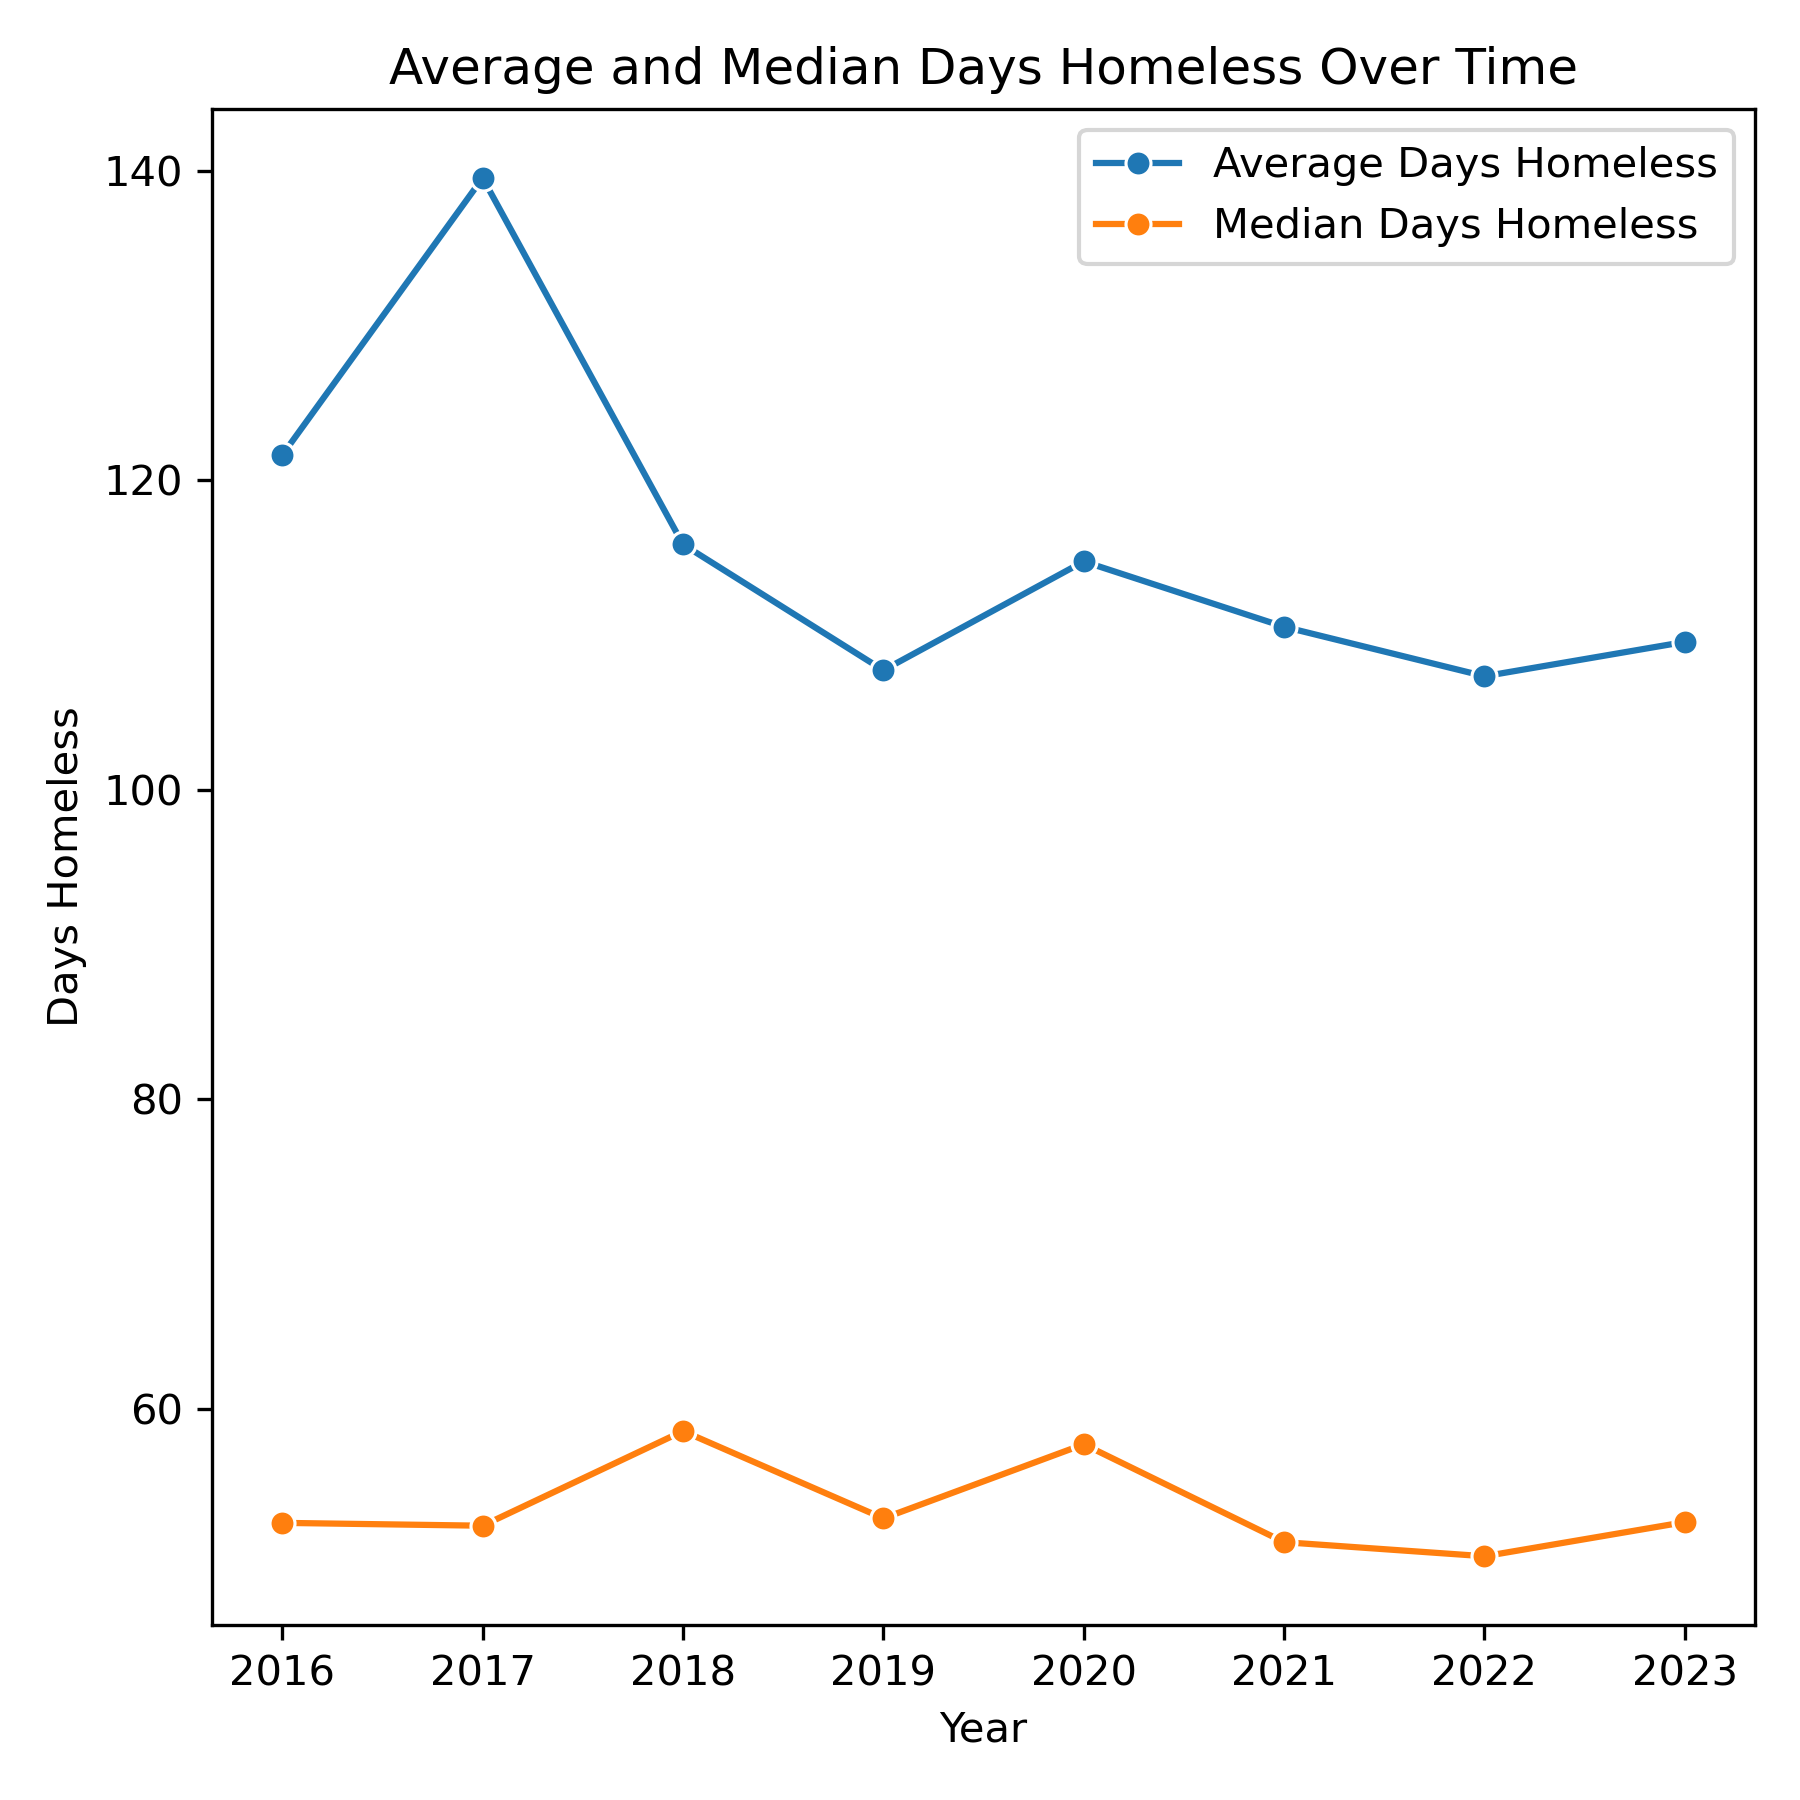
\includegraphics[width=0.48\linewidth]{graphs/days_homeless.png}
\caption{National Homelessness System Dynamics, 2016–2023}
\label{fig:national_trends}
\end{figure}

The onset of the COVID-19 pandemic in 2020 coincides with a sharp contraction in both inflows and exits. First-time homelessness entries declined substantially in 2020, falling by more than 100,000 relative to 2019. Exits from homelessness also declined sharply during this period, reflecting disruptions to housing markets, service provision, and shelter operations during the pandemic. In the years following 2020, both inflows and exits recover, rising steadily through 2023.

A notable feature of the post-pandemic period is that the pre-COVID gap between exits and inflows largely disappears. While exits exceeded inflows prior to 2020, the two series move much more closely together after the pandemic. By 2023, the number of individuals exiting homelessness is nearly equal to the number entering the system. This convergence suggests that the balance between entry and exit flows—central to the dynamics of homelessness systems—changed meaningfully during the pandemic period.

Measures of homelessness duration exhibit comparatively less variation over time. Both the average and median number of days individuals spend homeless fluctuate modestly across years, generally remaining within a relatively narrow range. This stability suggests that while the pandemic substantially affected the volume of flows into and out of homelessness systems, it did not dramatically alter the typical length of homelessness spells at the national level.

% ------------------------------------------------------------------------------
\section{Empirical Strategy}
% ------------------------------------------------------------------------------

\subsection{Dose-Response Framework}
To estimate the relationship between eviction moratoria and homelessness dynamics, I estimate a dose–response panel model exploiting variation in the intensity of eviction suppression across states and over time.

The baseline specification is:

\begin{equation}
Y_{st} = \alpha_s + \gamma_t + \theta \, \text{Dose}_{st} + X_{st}\beta + \varepsilon_{st},
\end{equation}

where $Y_{st}$ denotes a homelessness outcome in state $s$ and year $t$, $\alpha_s$ are state fixed effects, and $\gamma_t$ are year fixed effects. The variable $\text{Dose}_{st}$ measures the intensity of eviction moratoria in state $s$ at time $t$. The parameter $\theta$ captures the marginal effect of increased eviction suppression on homelessness outcomes.

State fixed effects absorb time-invariant differences across states, such as baseline housing market conditions or structural differences in homelessness service systems. Year fixed effects control for national shocks that affect all states simultaneously, including macroeconomic conditions and pandemic-related disruptions.

The vector $X_{st}$ includes time-varying controls capturing state-level economic conditions and pandemic severity. Standard errors are clustered at the state level throughout.

\subsection{Pre-Trends and Validation}

A key identifying assumption of the difference-in-differences design is that, absent eviction
moratoria, homelessness outcomes in treated and untreated Continuums of Care (CoCs) would
have followed parallel trends. Because all treated areas were exposed to eviction moratoria
beginning in the same calendar year (2020), a fully dynamic event-study specification with year
fixed effects is not separately identified. I therefore assess the plausibility of the parallel trends
assumption using a combination of descriptive evidence and regression-based pre-trend tests.

Figures \ref{fig:inflow_trends}–\ref{fig:duration_trends} plot mean homelessness inflows, total exits, and average days homeless over time for treated and never-treated CoCs. Across all three outcomes, treated and untreated areas exhibit relatively stable and similar trends prior to 2020, though levels differ substantially between the two groups. These level differences are absorbed by state fixed effects in the main specification and do not threaten identification.

Beginning in 2020, outcomes diverge sharply across groups. Treated CoCs experience increases
in inflows and total exits, alongside a gradual rise in average days homeless, while untreated
CoCs display sharp declines in exits and pronounced spikes in homelessness duration in 2020
followed by a rapid rebound. While these post-2020 patterns likely reflect the combined influence
of eviction moratoria and the COVID-19 pandemic, the absence of visible divergence prior to 2020
provides preliminary support for the parallel trends assumption.

\subsubsection{Regression-Based Pre-Trend Tests}

To formally test for differential pre-treatment trends, I estimate regressions of the form:
\begin{equation}
Y_{st} = \alpha_s + \gamma_t + \beta(\text{Treated}_s \times t) + \epsilon_{st}
\end{equation}
using only pre-2020 data, where $Y_st$ denotes the outcome of interest in state $s$ and year $t$, $\alpha_s$ are state fixed effects and $\gamma_t$ are year fixed effects. The coefficient $\beta$ captures whether treated states exhibit a systematically different linear trend prior to policy adoption. 

Table \ref{tab:pretrends} reports regression-based tests for differential pre-treatment trends using data from 2016–2019. For homelessness exits and median days homeless, the estimated interaction between treatment status and the linear time trend is small and statistically indistinguishable from zero. For homelessness inflows, the estimated pre-trend coefficient is negative and marginally statistically significant at the 10 percent level. The magnitude of this estimate implies that treated states experienced a modestly faster decline in inflows prior to the pandemic relative to control states. However, the estimated difference is small relative to the overall scale of inflow variation.

Moreover, the main empirical specification exploits variation in the intensity and duration of eviction protections across states and over time rather than relying solely on a treated-versus-untreated comparison. As a result, identification primarily comes from differences in policy strength within states during the pandemic period. Taken together, these results provide limited evidence of differential pre-treatment trends and do not appear to materially threaten the identification strategy.

% ------------------------------------------------------------------------------
\section{Results}
% ------------------------------------------------------------------------------

Tables \ref{tab:inflow}--\ref{tab:median_days} present estimates from the dose–response specification relating eviction moratoria to homelessness system outcomes. Each column reports the coefficient on a different measure of eviction policy strength: the share of the year in which a moratorium was active, the Princeton Eviction Lab Housing Policy Scorecard, and a composite measure of moratorium intensity that combines duration and policy strength. All specifications include state and year fixed effects, and standard errors are clustered at the state level.

\subsection{Homelessness Inflows}

\begin{table}
\centering
\begin{threeparttable}
\caption{Eviction Moratoria and Homelessness Inflows}
\label{tab:inflow}
\begin{tabular}{lccc}
\toprule
 & \shortstack{\\[0.1ex] Share of Year \\ with Active Moratorium} & \shortstack{\\[0.1ex] Housing Policy \\ Scorecard} & Moratorium Intensity \\
\midrule
Beta & -49.915** & -6.419* & -20.926*** \\
Observations & 415 & 415 & 415 \\
State FE & Yes & Yes & Yes \\
Year FE & Yes & Yes & Yes \\
Within $R^2$ & 0.139 & 0.113 & 0.151 \\
\bottomrule
\end{tabular}

\begin{tablenotes}[flushleft]
\footnotesize
\item \textit{Notes:} Each cell reports the coefficient on the policy measure listed in the column header from a separate regression of homelessness inflow (first-time homeless per 1,000 population). All regressions include state and year fixed effects with standard errors clustered at the state level.
\end{tablenotes}
\end{threeparttable}
\end{table}

Table \ref{tab:inflow} reports results for inflows into the homelessness system, measured as the number of individuals entering homelessness for the first time per 1,000 residents. Across all three policy measures, stronger eviction moratoria are associated with statistically significant reductions in homelessness inflows. 

Using the share-of-year specification, a full year of eviction protections is associated with approximately 50 fewer first-time homeless entries per 1,000 residents. Similarly, higher values of the Eviction Lab scorecard—which captures the strength of eviction protections—are associated with lower inflows. The composite moratorium intensity measure yields the strongest statistical relationship, indicating that both the duration and the strictness of eviction restrictions are negatively correlated with entry into homelessness. 

These results are consistent with the primary mechanism through which eviction moratoria were intended to operate: by preventing housing loss, eviction restrictions reduce the flow of households entering homelessness.

\subsection{Homelessness Exits}

\begin{table}[H]
\centering
\begin{threeparttable}
\caption{Eviction Moratoria and Homelessness Exits}
\label{tab:exits}
\begin{tabular}{lccc}
\toprule
 & \shortstack{\\[0.1ex] Share of Year \\ with Active Moratorium} & \shortstack{\\[0.1ex] Housing Policy \\ Scorecard} & Moratorium Intensity \\
\midrule
Beta & -40.018** & -9.866*** & -15.518*** \\
Observations & 415 & 415 & 415 \\
State FE & Yes & Yes & Yes \\
Year FE & Yes & Yes & Yes \\
Within $R^2$ & 0.076 & 0.088 & 0.084 \\
\bottomrule
\end{tabular}

\begin{tablenotes}[flushleft]
\footnotesize
\item \textit{Notes:} Each cell reports the coefficient on the policy measure listed in the column header from a separate regression of homelessness exits (number of homelessness exits per 1,000 population). All regressions include state and year fixed effects with standard errors clustered at the state level.
\end{tablenotes}
\end{threeparttable}
\end{table}

Table \ref{tab:exits} presents results for exits from the homelessness system. Alongside the inflow results, stronger eviction moratoria are also associated with statistically significant reductions in exits from homelessness. 

This pattern is somewhat less straightforward to interpret. One possibility is mechanical: if fewer individuals enter the homelessness system during periods of stronger eviction protections, there may simply be fewer individuals available to exit. Another possibility is that pandemic-related disruptions—such as social distancing requirements in shelters or slower administrative processing—reduced the efficiency of rehousing programs during the same period. 

A third mechanism relates to housing market conditions. If eviction moratoria reduced turnover in the rental housing stock, this may have lowered the availability of vacant units into which individuals experiencing homelessness could be rehoused, thereby slowing exit rates.

\subsection{Duration of Homelessness}

\begin{table}[H]
\centering
\begin{threeparttable}
\caption{Eviction Moratoria and Homelessness Duration}
\label{tab:median_days}
\begin{tabular}{lccc}
\toprule
 & \shortstack{\\[0.1ex] Share of Year \\ with Active Moratorium} & \shortstack{\\[0.1ex] Housing Policy \\ Scorecard} & Moratorium Intensity \\
\midrule
Beta & -16.918 & -2.927* & -3.680* \\
Observations & 415 & 415 & 415 \\
State FE & Yes & Yes & Yes \\
Year FE & Yes & Yes & Yes \\
Within $R^2$ & 0.013 & 0.011 & 0.009 \\
\bottomrule
\end{tabular}

\begin{tablenotes}[flushleft]
\footnotesize
\item \textit{Notes:} Each cell reports the coefficient on the policy measure listed in the column header from a separate regression of homelessness duration (median days homeless). All regressions include state and year fixed effects with standard errors clustered at the state level.
\end{tablenotes}
\end{threeparttable}
\end{table}

An an attempt to shed light on these mechanisms, Table \ref{tab:median_days} examines the relationship between eviction moratoria and the median duration of homelessness spells. If the decline in exits reflected worsening congestion within homelessness systems, one would expect median days homeless to increase during periods of stronger eviction protections. 

Instead, the estimated coefficients are small and negative, and only marginally statistically significant in two specifications. While the point estimates suggest slightly shorter homelessness spells in states with stronger eviction protections, the effects are economically modest and the explanatory power of these regressions is low. 

Taken together, these results suggest that the observed reduction in exits is unlikely to reflect a large increase in congestion within homelessness systems. One interpretation is that states implementing stronger eviction protections may also have had more developed or better-resourced homelessness service systems, allowing them to maintain relatively stable rehousing timelines despite pandemic disruptions.

\subsection{Interpretation}

Overall, the results indicate that stronger and longer eviction moratoria are strongly associated with reductions in entries into homelessness systems, consistent with the intended purpose of these policies. At the same time, exits from homelessness also decline during periods of stronger eviction protection, though the mechanisms underlying this pattern are less clear. 

The absence of a corresponding increase in homelessness duration suggests that the reduction in exits does not primarily reflect growing system congestion. Instead, the results point toward a combination of reduced inflows and broader pandemic-related housing market dynamics affecting the operation of homelessness systems during this period.


% ------------------------------------------------------------------------------
\clearpage
\bibliographystyle{apalike}  % or econ-style if you prefer
\bibliography{references}

% ------------------------------------------------------------------------------


\clearpage
\appendix

\nociteW{*}

\bibliographystyleW{apalike}
\bibliographyW{reading_wishlist}

% ------------------------------------------------------------------------------
\section{Tables \& Figures}
% ------------------------------------------------------------------------------
  \begin{figure}[!htbp]\centering
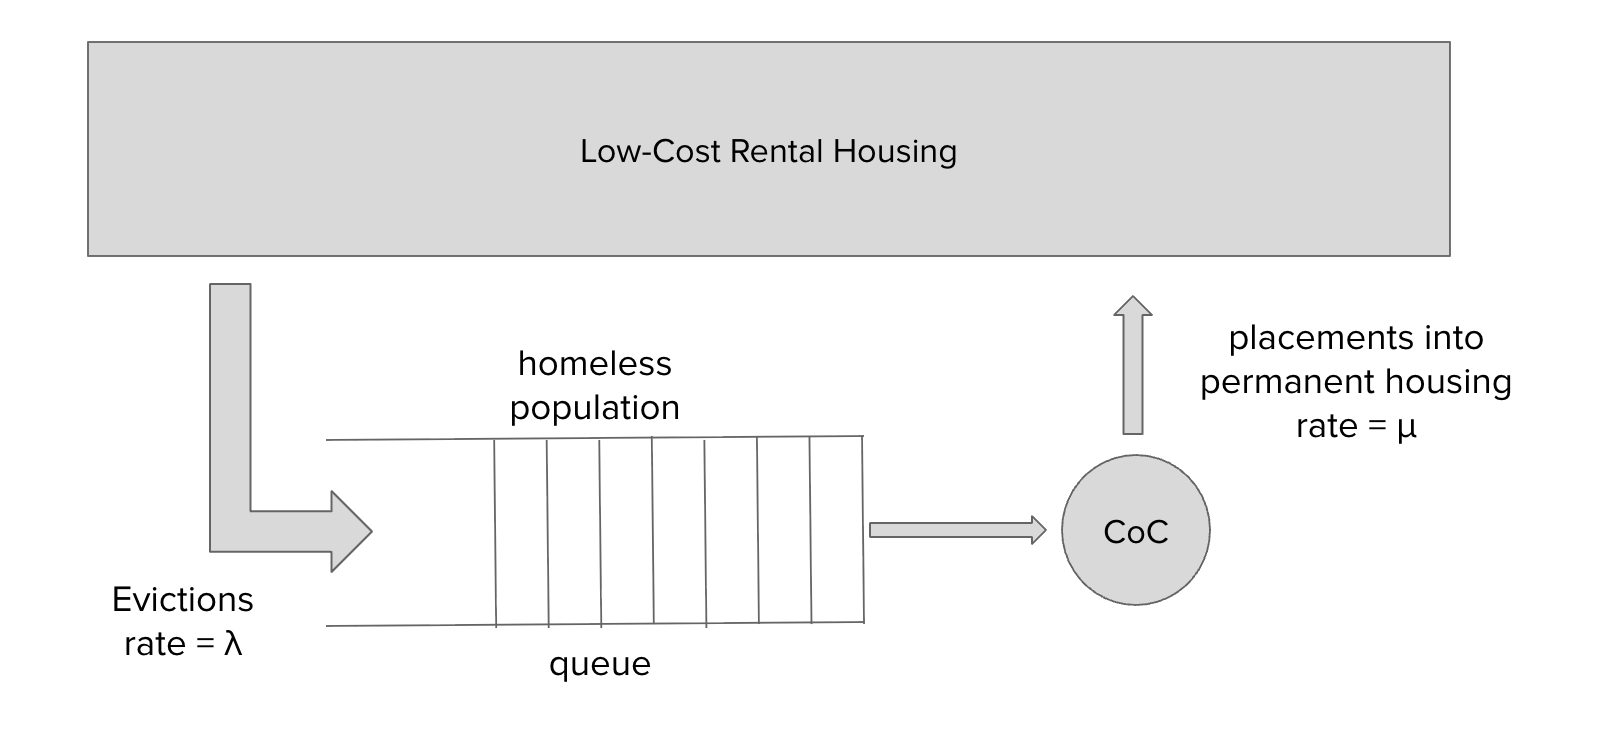
\includegraphics[width=0.75\textwidth]{graphs/queue.png}
\caption{A Queuing View of Homelessness}
\label{fig:queue}
\end{figure}

\begin{figure}[!htbp]\centering
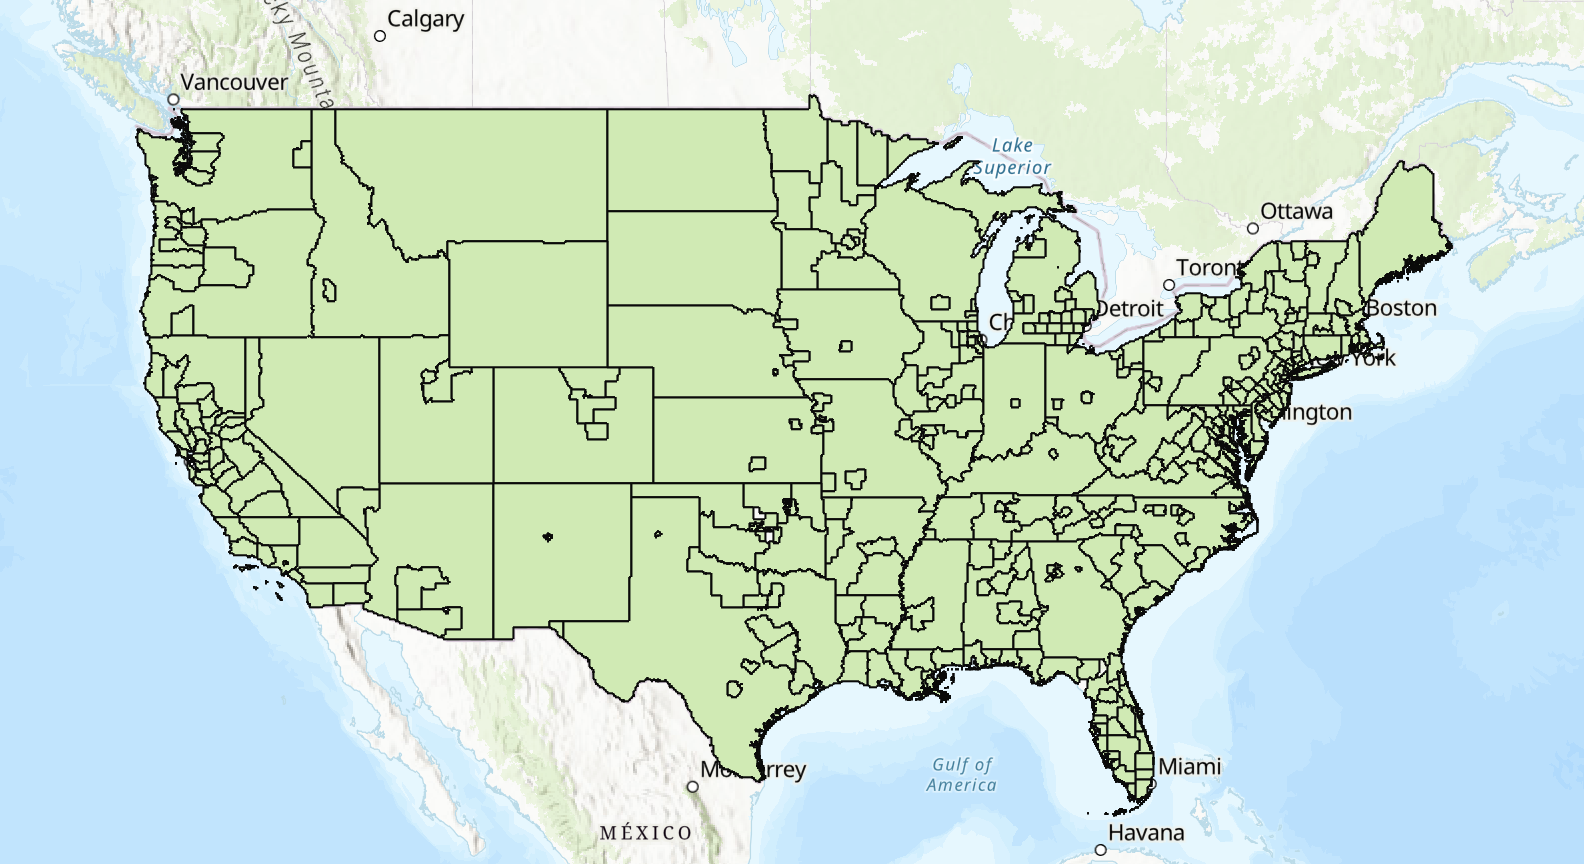
\includegraphics[width=1\textwidth]{graphs/coc_map.png}
\caption{Map of Continuums of Care}
\label{fig:coc_map}
\end{figure}

\begin{figure}[!htbp]\centering
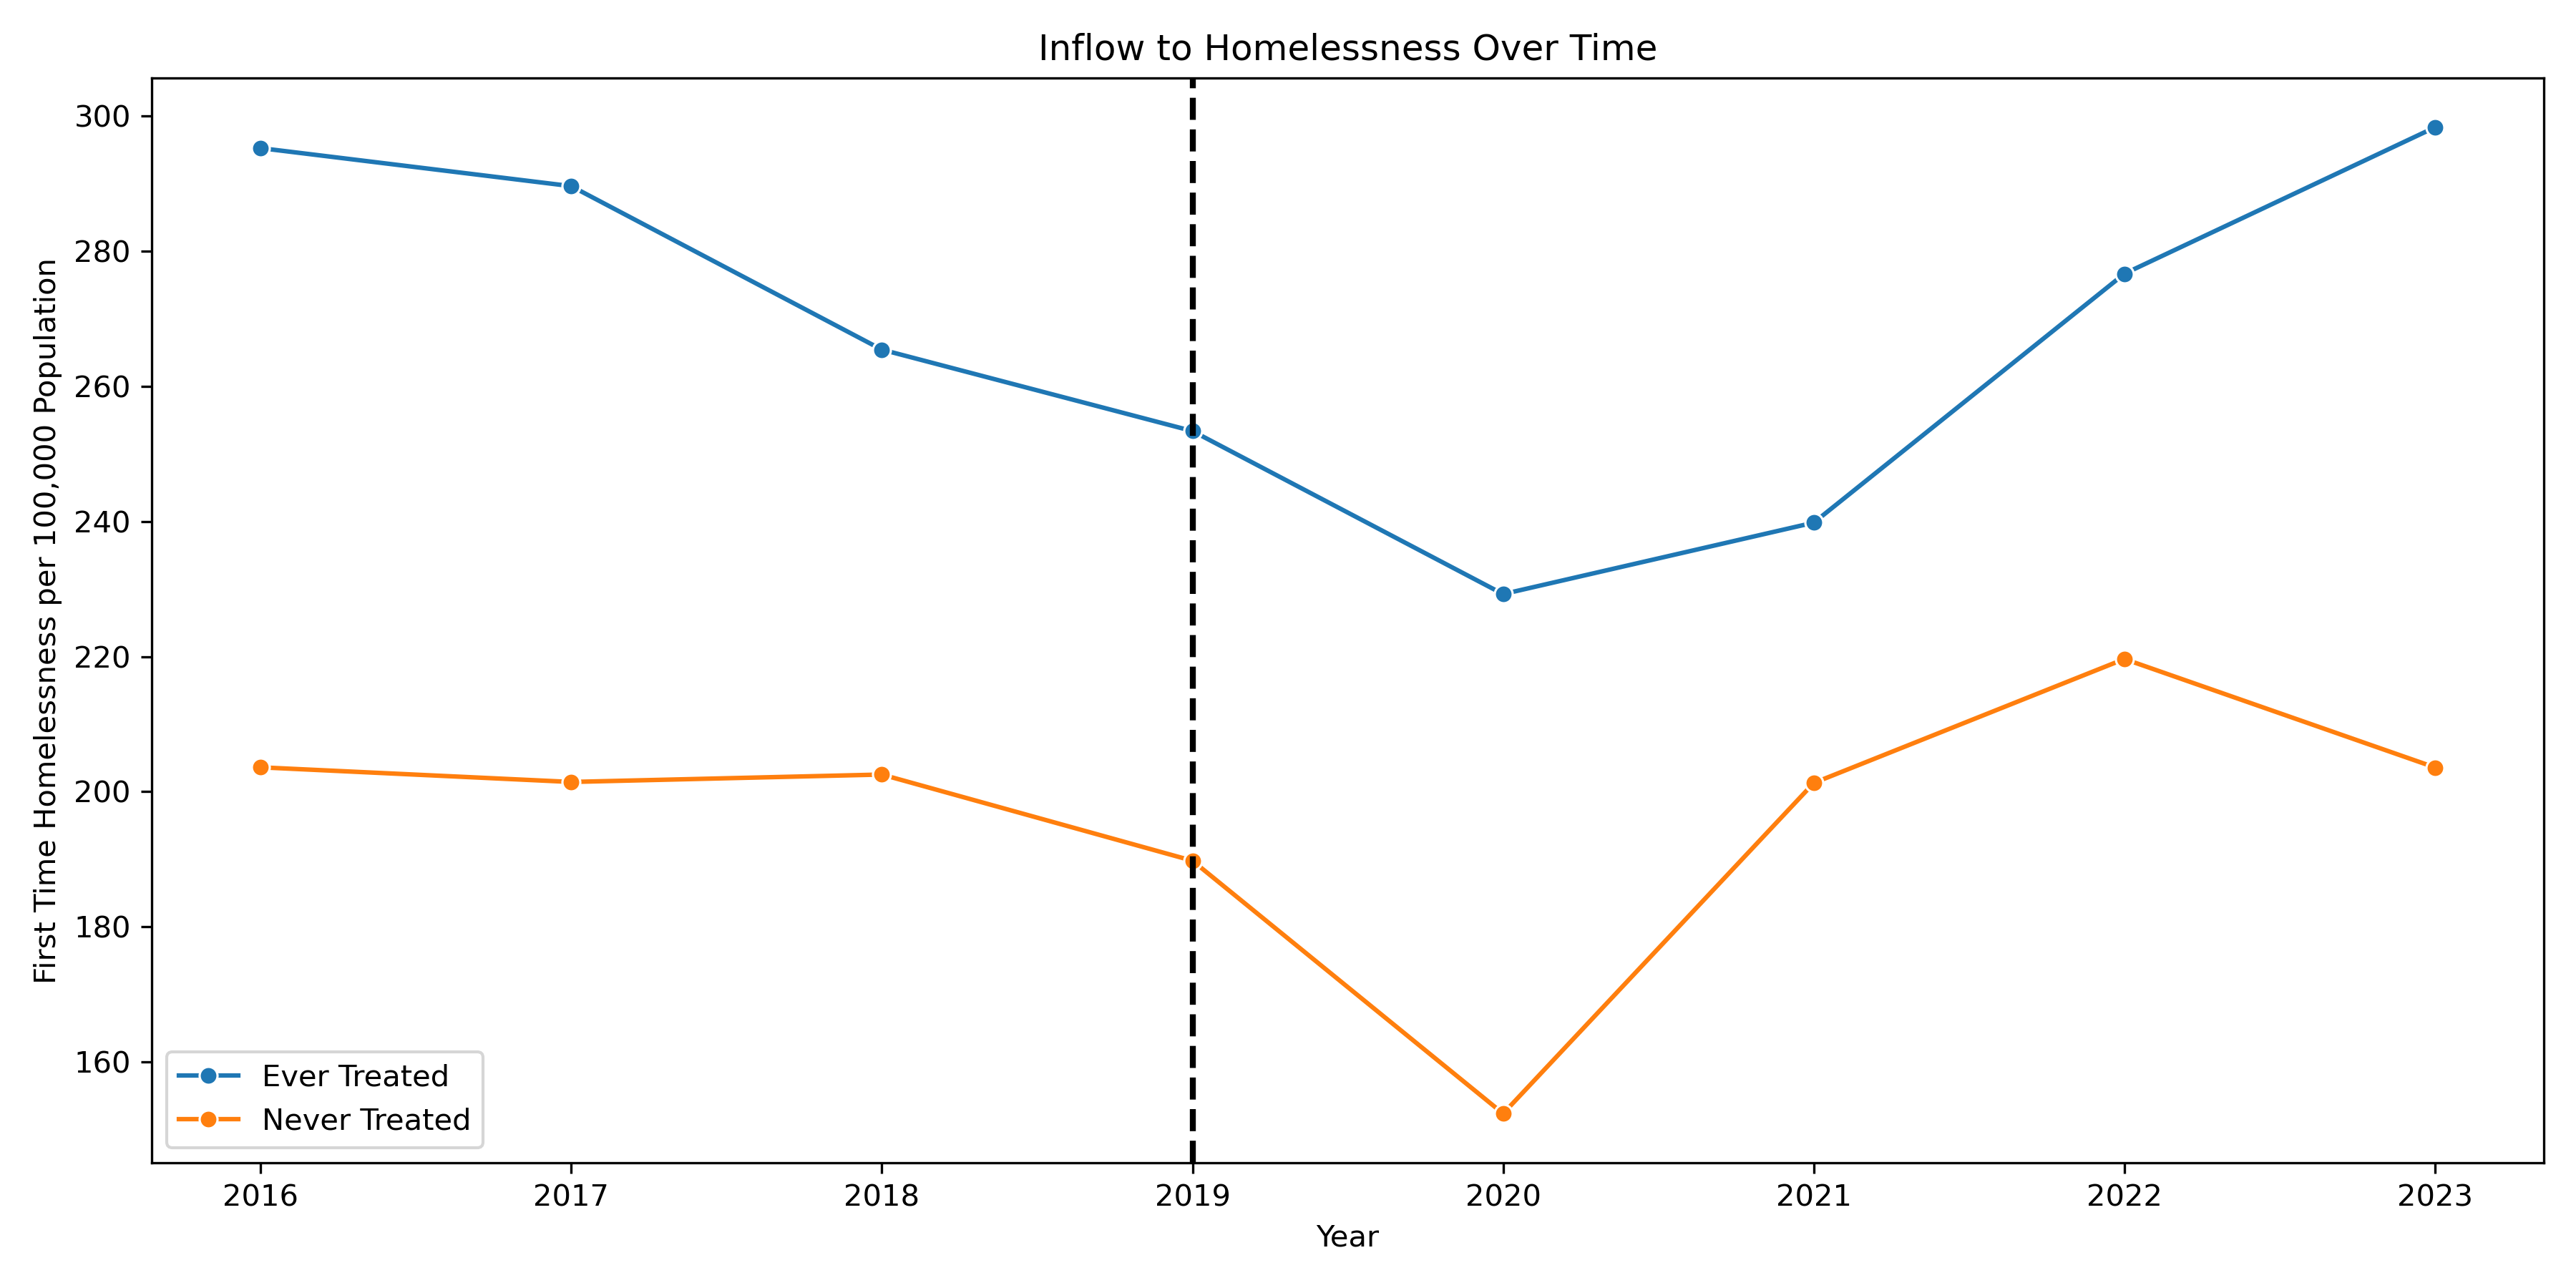
\includegraphics[width=0.5\textwidth]{graphs/inflow_trends_state.png}
\caption{Mean Homelessness Inflow by Treatment Status}
\label{fig:inflow_trends}
\end{figure}

\begin{figure}[!htbp]\centering
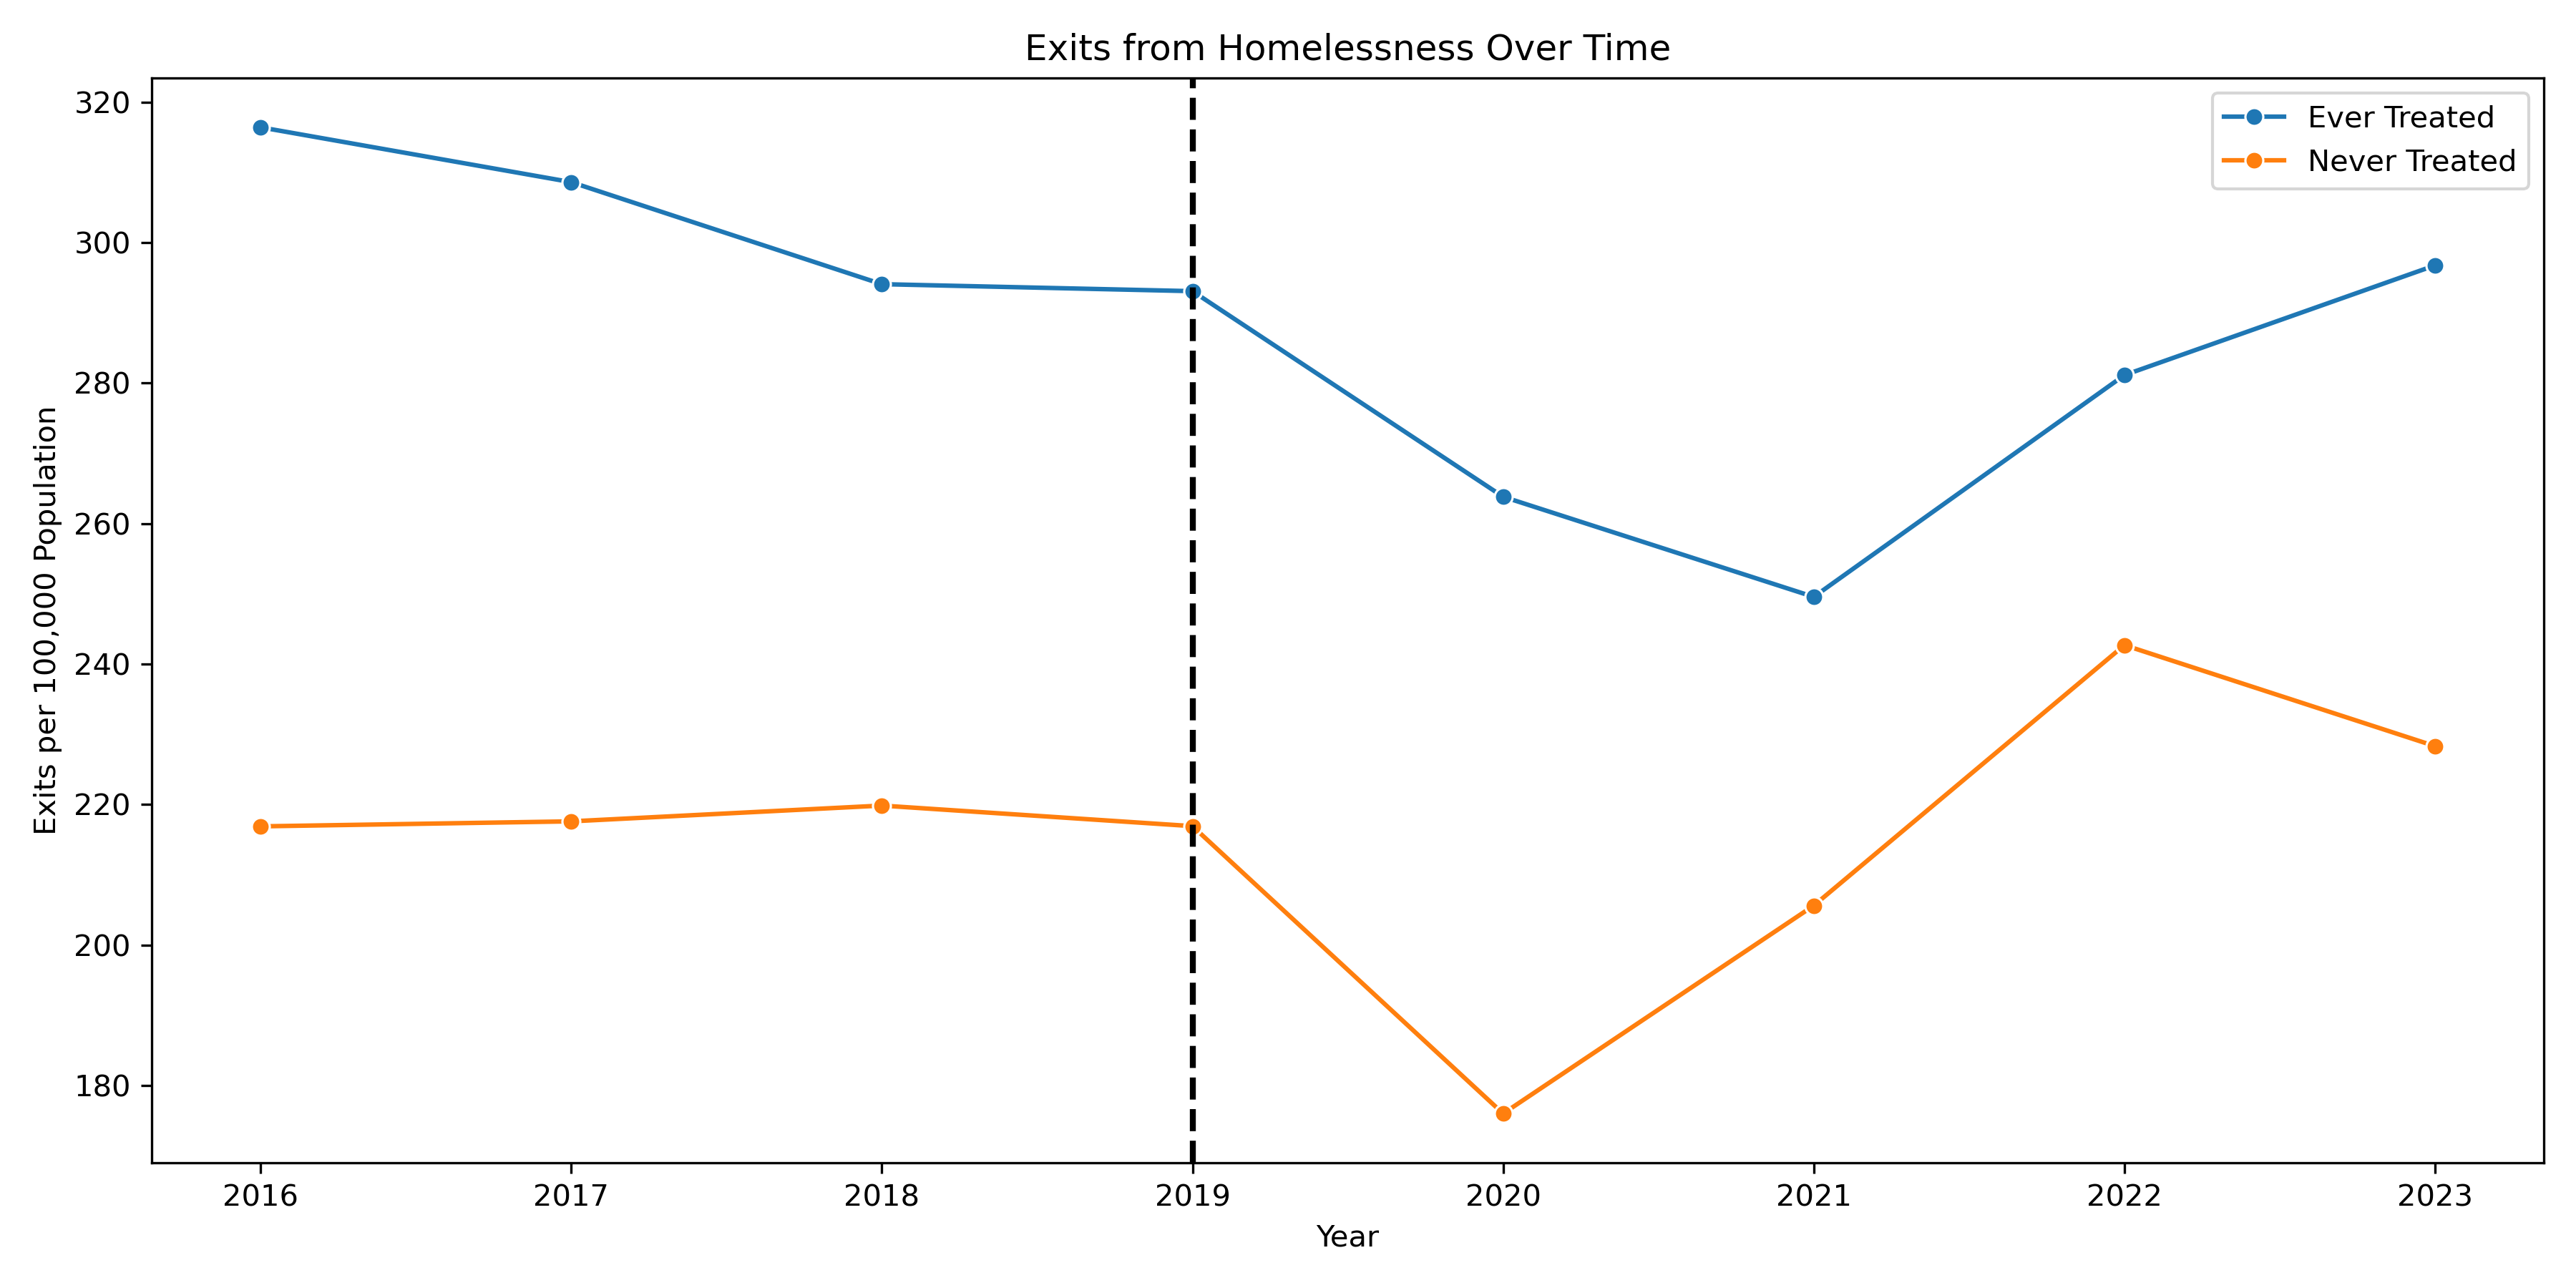
\includegraphics[width=0.5\textwidth]{graphs/exits_trends_state.png}
\caption{Mean Total Exits from Homelessness by Treatment Status}
\label{fig:exits_trends}
\end{figure}

\begin{figure}[!htbp]\centering
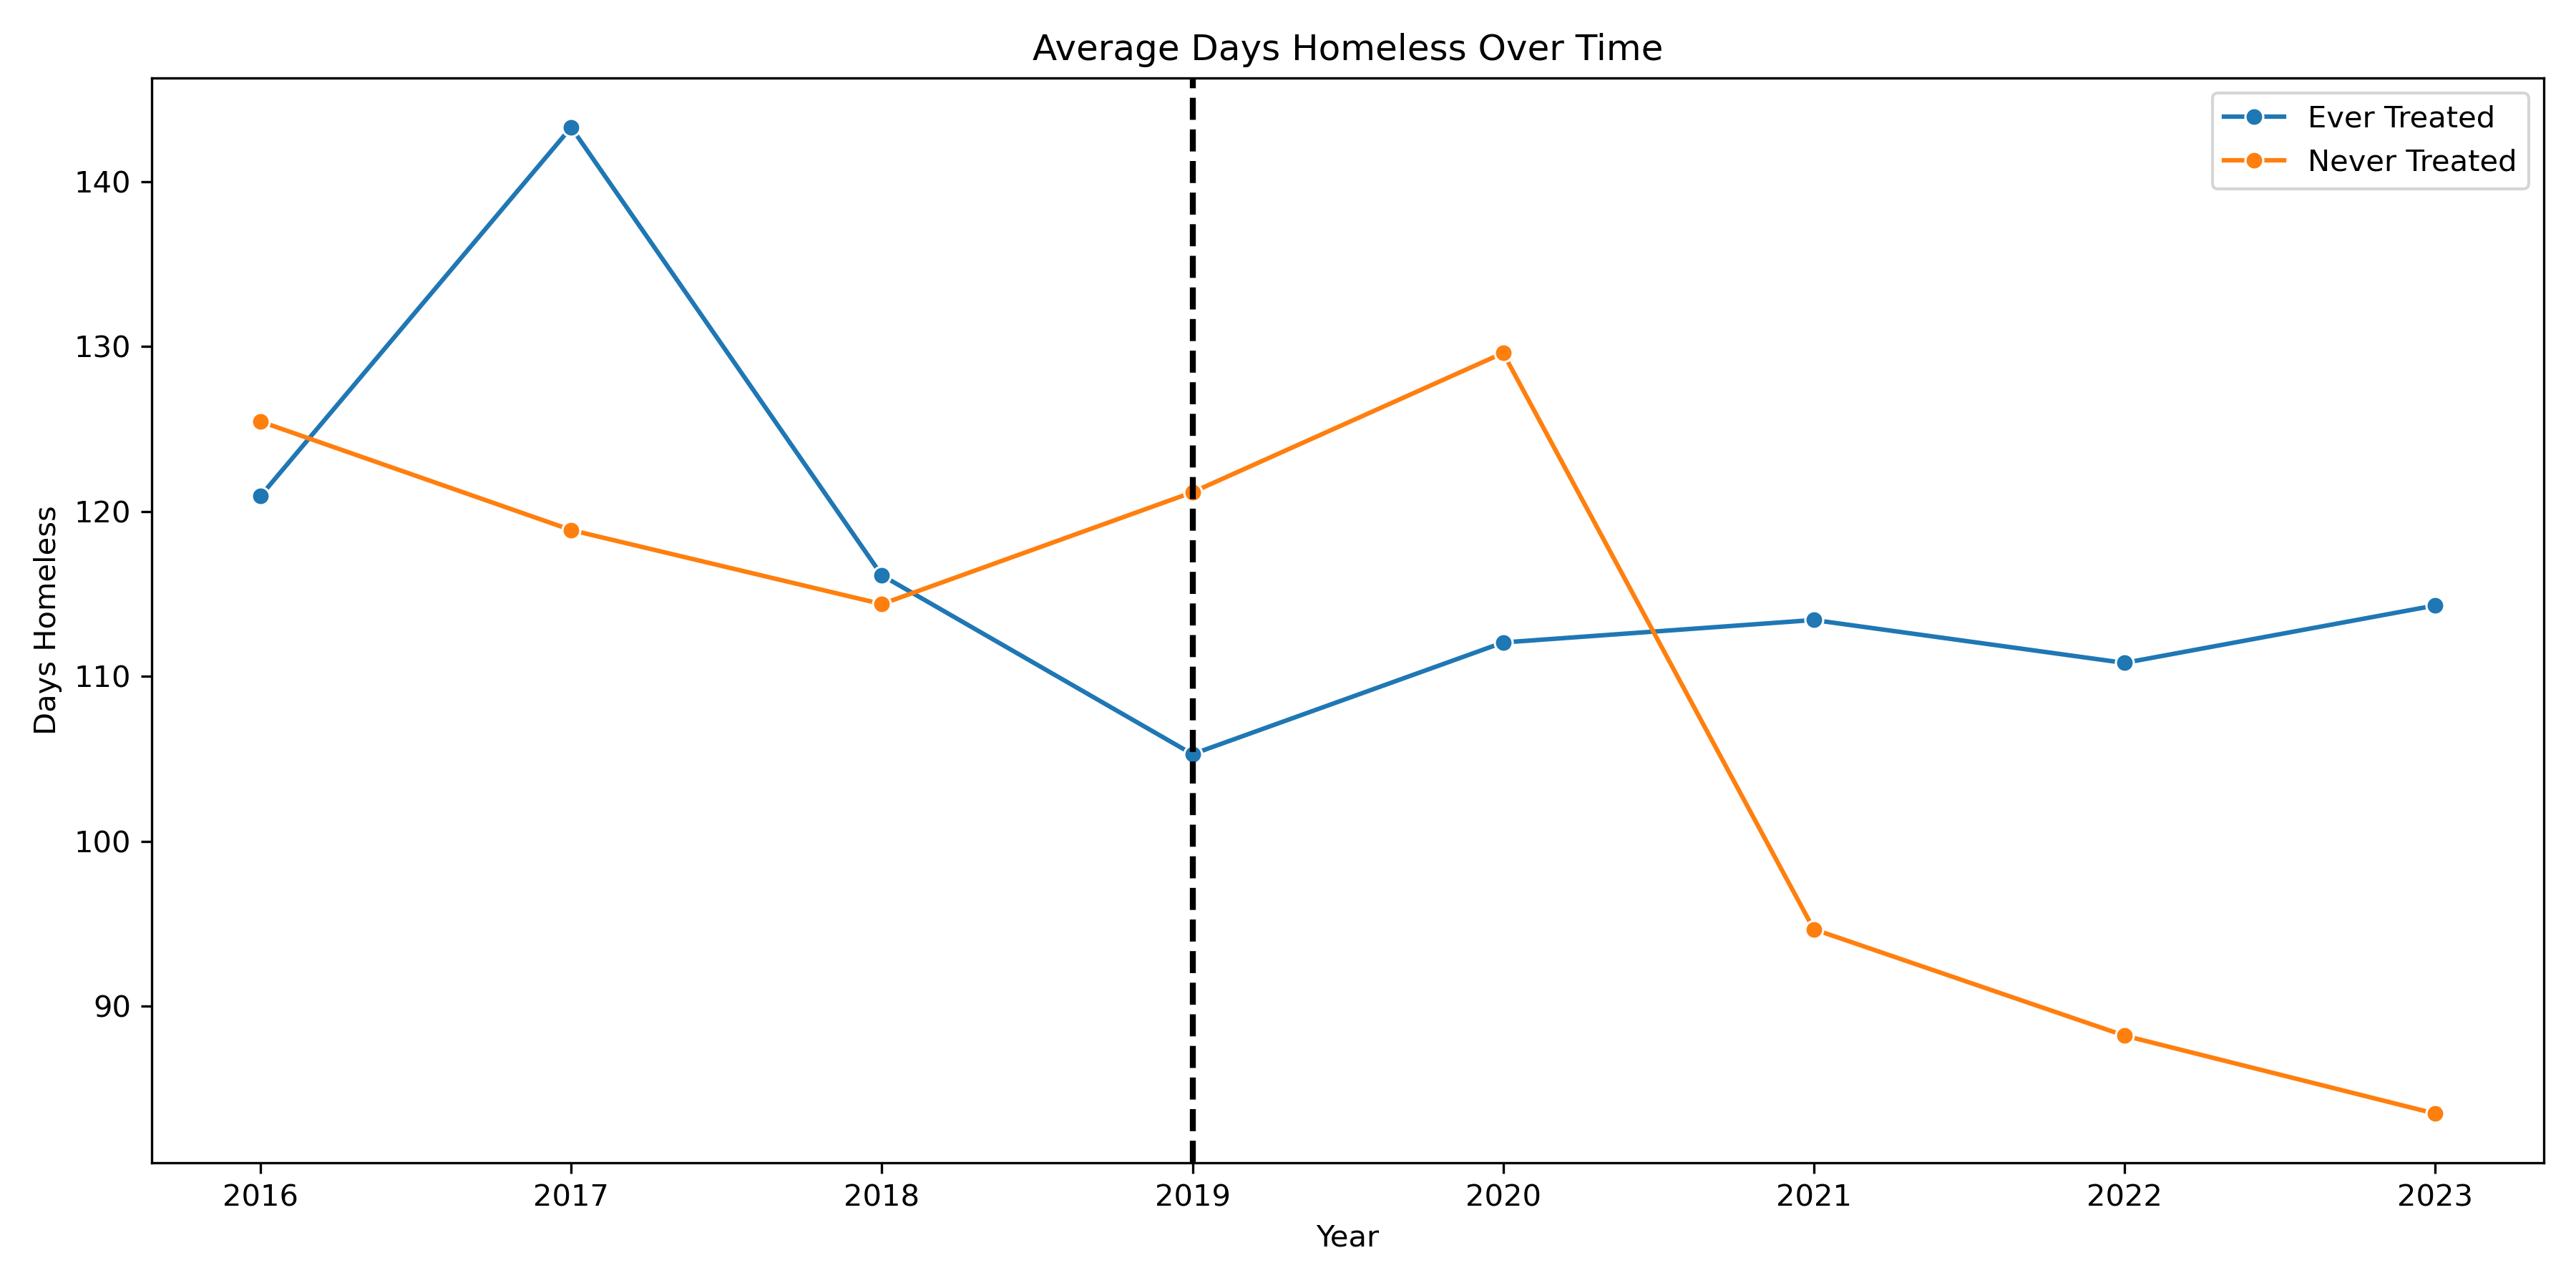
\includegraphics[width=0.5\textwidth]{graphs/days_homeless_trends_state.png}
\caption{Mean Average Days Homeless by Treatment Status}
\label{fig:duration_trends}
\end{figure}

\begin{table}[!htbp]\centering
\caption{Differential Pre-Trend Tests}
\label{tab:pretrends}
\begin{tabular}{lccc}
\toprule
 & Inflow & Exits & Median Days Homeless \\
\midrule
Ever Treated $\times$ Linear Time Trend & -122.152 & 28.847 & -5.452 \\
 & (245.455) & (255.965) & (7.101) \\
Observations & 208 & 208 & 208 \\
State FE & Yes & Yes & Yes \\
Year FE & Yes & Yes & Yes \\
Within $R^2$ & 0.040 & -0.005 & -0.062 \\
\bottomrule
\end{tabular}

\begin{flushleft}
\footnotesize
Notes: Each column reports a regression of the outcome on a linear calendar-year trend interacted with treatment status, estimated using pre-2020 data only. All specifications include Continuum of Care and year fixed effects. Standard errors are clustered at the state level.
\end{flushleft}
\end{table}


\end{document}
